\documentclass[10pt]{article}
%\documentclass[10pt]{book}

\usepackage[draft]{fixme}

\usepackage{listings}
\usepackage{html}
\usepackage{color}
\usepackage{multicol}
\usepackage{multirow}
\usepackage{graphicx}
\usepackage{alltt}
% style for code listing
\lstset{language={C},basicstyle=\scriptsize} 
\newcommand{\hlstd}[1]{\textcolor[rgb]{0,0,0}{#1}}
\newcommand{\hlkey}[1]{\textcolor[rgb]{0,0,0}{\bf{#1}}}
\newcommand{\hlnum}[1]{\textcolor[rgb]{0.16,0.16,1}{#1}}
\newcommand{\hltyp}[1]{\textcolor[rgb]{0.51,0,0}{#1}}
\newcommand{\hlesc}[1]{\textcolor[rgb]{1,0,1}{#1}}
\newcommand{\hlstr}[1]{\textcolor[rgb]{1,0,0}{#1}}
\newcommand{\hldstr}[1]{\textcolor[rgb]{0.51,0.51,0}{#1}}
\newcommand{\hlcom}[1]{\textcolor[rgb]{0.51,0.51,0.51}{\it{#1}}}
\newcommand{\hldir}[1]{\textcolor[rgb]{0,0.51,0}{#1}}
\newcommand{\hlsym}[1]{\textcolor[rgb]{0,0,0}{#1}}
\newcommand{\hlline}[1]{\textcolor[rgb]{0.33,0.33,0.33}{#1}}

\newcommand{\mySmallFontSize}{\scriptsize}
\newcommand{\mySmallestFontSize}{\tiny}

\newcommand{\codeFontSize}{\scriptsize}
\newcommand{\code}[1]{{\scriptsize #1}}

% Software version number
%\newcommand{\VersionNumber}{@VERSION@}

%\newcommand{\ExampleDirectory}{@top_srcdir@/projects/compass/tests}

% Latex trick to allow us to comment out large sections of documentation
\newcommand{\commentout}[1]{}

% change the title of the Fixme List
\renewcommand{\listfixmename}{Things to Fix in Documentation}

\newcommand{\comm}[2]{\bigskip
                      \begin{tabular}{|p{11cm}|}\hline
                      \multicolumn{1}{|c|}{{\bf Comment by #1}}\\ \hline
                      #2\\ \hline
                      \end{tabular}
                      \bigskip
                     }

\def\verbatimfile#1{\begingroup
                    \@verbatim \frenchspacing \@vobeyspaces
                    \input#1 \endgroup
}

\newcounter{lineno}

% Taken from verbatimfiles.sty on web
\makeatletter %JCL

\def\verbatimlisting#1{\setcounter{lineno}{0}%
    \begingroup \@verbatim \frenchspacing \@vobeyspaces \parindent=20pt
    \everypar{\stepcounter{lineno}\llap{\thelineno\ \ }}\input#1
    \endgroup
}

\makeatother %JCL

% \endinput

\addtolength{\textheight}{0.5in}
\sloppy

%---------------------------------------------------------------------
% Begin Document
%---------------------------------------------------------------------

\begin{document}

% This draft mode eliminates the figures (leaves boxes for where they would be)
%\textcolor{green}{(Associated with ROSE Version @VERSION@)} } }
%\psdraft

\title{ {\bf \textcolor{red}{A Compiler-Independent Many-Core Runtime System} \\ 
              \textcolor{blue}{Draft User Tutorial} \\
              } }
\author{ {\bf ROSE Team} \\
         Lawrence Livermore National Laboratory \\ 
         Livermore, CA  94550 \\
         925-423-2668 (office)  925-422-6278 (fax) \\
         \{liao6, quinlan1\}@llnl.gov \\
         Project Web Page:
         \htmladdnormallink{http://www.rosecompiler.org}{http://www.rosecompiler.org} \\
         UCRL Number for ROSE User Manual: UCRL-SM-210137-DRAFT \\
         UCRL Number for ROSE Tutorial: UCRL-SM-210032-DRAFT \\
         UCRL Number for ROSE Source Code: UCRL-CODE-155962 \\ \\
         \htmladdnormallink{ROSE User Manual
         (pdf)}{http://www.rosecompiler.org/ROSE_UserManual/ROSE-UserManual.pdf} \\
         \htmladdnormallink{ROSE Tutorial
         (pdf)}{http://www.rosecompiler.org/ROSE_Tutorial/ROSE-Tutorial.pdf} \\
         \htmladdnormallink{ROSE HTML Reference (html
         only)}{http://www.rosecompiler.org/ROSE_HTML_Reference/index.html}
       }
\maketitle
\newpage


% This fixes the really long table of contents problem
\setcounter{tocdepth}{2}

\tableofcontents
\newpage
%

\chapter{Introduction}

\section{Overview}

\label{introduction::overview}

   Compass is a tool for the checking of source code.  It is
based on the ROSE compiler infrastructure and demonstrates to
use of ROSE to build lots of simple pattern detectors for analysis
of C, C++, and Fortran source code.

   The purpose of this work is several fold:
\begin{itemize}
   \item Provide a concrete tool to support interactions with lab customers.
   \item Provide a home for the security analysis specific detectors being built within
         external research projects.
   \item Provide an external tool for general analysis of software.
   \item Provide a tool to support improvements to the ROSE source code base.
   \item Define an infrastructure for an evolving and easily tailored program analysis tool.
   \item Provide a simple motivation for expanded use of ROSE by external users.
         Development, testing, and evaluation of ROSE infrastructure is best facilitated 
         through its expanded use by others and this provides a specific and attractive
         tool that can provide feedback to users about their own code projects.  Even
         though optimization research is our focus, this gets our supporting
         infrastructure for optimization research out and into use by others in the form
         of an extensible tool.
\end{itemize}

   Note that as the collection of detectors grows we will periodically reorganize the 
collection.  At some point soon we will build a hierarchy to organize the evolving
collection.

%\subsection{A basis for other source analysis tools}
\paragraph{A basis for other source analysis tools}
   Input and output to ROSE is organized so that any number of source could be used.
So although we provide a compiler interface (for simplicity), we will also provide a 
GUI interface as an alternative interface to demonstrate that the detectors are orthogonal
to there use in alternative tools.  Alternative tool interfaces should be possible 
and will further demonstrate the independence of the input and output mechanisms to
the designs and implementation of the core detectors.

\paragraph{Add Your Own Detector}

    Detectors written in Compass make direct use of ROSE and are 
designed to be copied and extended by users to develop their own 
detectors. We welcome the contribution of these detectors back to 
the ROSE team for inclusion into future releases of Compass;
full credit for all work will be provide to all authors.
Compass is an open source project using ROSE, an open source
compiler infrastructure.

    Each of the detectors are examples of how to
add your own detector to {\bf Compass}.  If you
build a detector that you would like to have be 
distributed with {\bf Compass}, please send it to
us and we will add your as an external contributor.

  Guidelines for contributions:
\begin{itemize}
   \item Use any Compass detector and an example.
   \item provide the documentation about your detector.
   \item Use any features in ROSE to support your detector; AST, Control Flow graph,
    System dependence Graph, Call Graph, Class Hierarchy Graph, etc.
   \item Your detector should have {\bf NO} side-effects on the AST.
\end{itemize}






\chapter{Design}


\section{Use Cases}

\label{design::UseCase}

Figure~\ref{Compass_usecase} shows the use cases of \emph{Compass}.
Compass as a tool is used to analyze source code. The analysis is triggered by the user who
selects which detectors to execute. The user also specifies the source code to be checked.
Results of the analysis are presented to that user.

\begin{figure}[th]
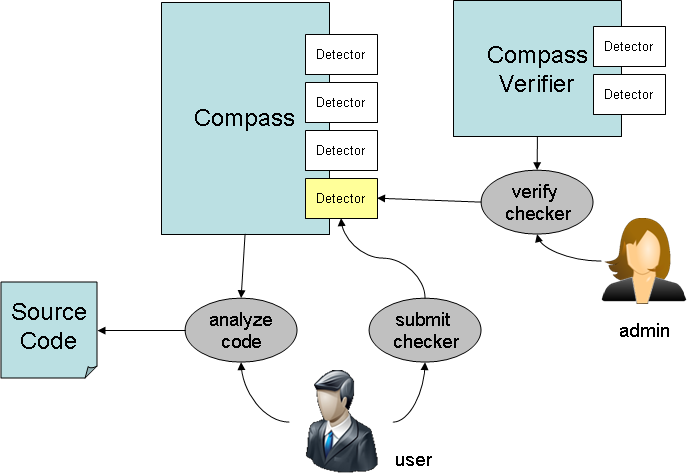
\includegraphics[width=4.5in]{compass_pic.png}
\caption{Compass Use Case}
\label{Compass_usecase}
\end{figure}

Furthermore, a user may contribute with his own detectors that he can add to Compass. Since 
external users may contribute detectors automatically via scripts, a verification of the 
validity and safety of these detectors is necessary. We provide a \emph{Compass Verifier}
that helps to check that all detectors are safe. Currently, the verifier is run by
a administrative person but may run automatically in the future.



\section{Design}

\begin{figure}[thb]
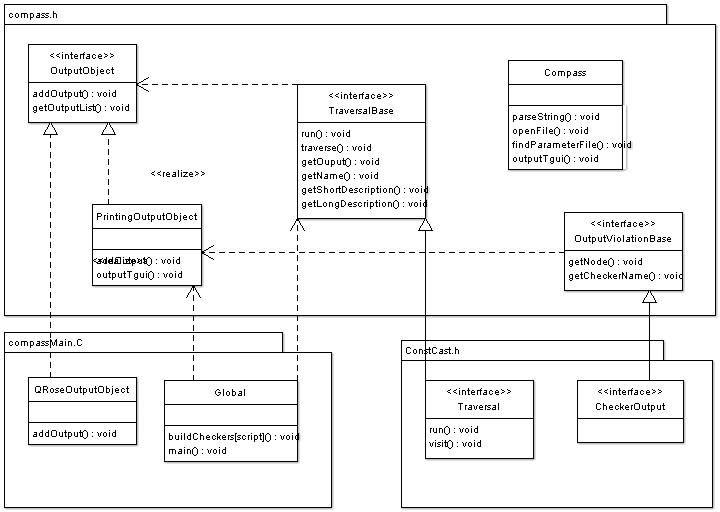
\includegraphics[width=6.0in]{compassdesign.png}
\caption{Compass Design}
\label{CompassDesign}
\end{figure}

Compass is designed to be easy to extend. Any user may write a detector and add it to Compass. Figure~\ref{CompassDesign}
illustrates the UML design decisions behind Compass.


Most of the functionality of Compass is in abstract classes hidden in the Compass namespace within compass.h - a file within
the compassSupport directory. All detectors, such as ConstCast illustrated in the figure, utilize the abstract classes
to traverse a program with all its nodes and to output violations found in that code according to the local algorithm.

CompassMain is the main executable that initially calls ROSE to parse a program. Then \emph{buildCheckers} is called to
load all detectors that are specified within a configuration file. The configuration file allows users to turn on and off
specific detectors for their run-time analyses. However, the configuration file only permits detectors to be loaded that 
were part of Compass at compile-time.

The main interface file compass.h contains the abstract classes \emph{TraversalBase} and 
\emph{OutputObject}. TraversalBase is the interface to ROSE, allowing a detector to traverse the ROSE AST (program) and hence
perform analysis on that AST. OutputObject aids to output defects found by a specific detector. More functionality to handle
e.g. file input and parameters provided to Compass, is provided within the Compass namespace.


\section{Compass Verifier}

\subsection{Threats} 

Compass must be safe, so that analyses and their results can be trusted. 
The main threats to the validity of Compass are:

\begin{itemize}
\item \emph{Malicious User}. A malicious user is an external user of Compass contributing a detector that performs malicious behaviour.  
\item \emph{Malicious Detector}. Compass is extensible and new detectos can be added externally (users outside the main development group).
  A detector can be programmed arbitrarily using the C/C++ and assembly programming languages. 
  It is therefore possible for a skilled programmer to hide malicious operations within a detector, e.g. allow a detector to scan the host machine and
  send data away. Compass must prevent detectors with malicious behaviour to be part of the Compass system. 
\item \emph{Source Code Replacement}. It should not be possible for users to exchange the source code of detectors within a running system,
  i.e. Compass cannot implement dynamic loading of detectors. Such a feature would compromise its safety.
\item \emph{Binary Replacement}. Another threat is the replacement of a valid Compass detector with a modified malicious version within a binary release of Compass.
  Therefore, Compass should be aware if parts of itself were modified and should not execute.
\end{itemize} 

\subsection{Safety Handling}

Compass is designed to be safe. The Compass Verifier is a stable separate copy of Compass that contains only a few detectors
to check (external and internal) user delivered detectors for safety. We have designed Compass in a way that it addresses the threats mentioned above:

\begin{itemize}
\item \emph{Malicious User}. Initially, we permit only trusted individuals to add new detectors to Compass. Once the verification process
  is matured, we will extend this policy to allow arbitrary users to contribute to Compass. 

\item \emph{Malicious Detector}. To prevent Compass to execute malicious code, the Compass Verifier executes its own detectors on
any user defined detector that is beeing considered to be added to Compass.
Currently, the Compass Verifier contains three detectors:

\begin{itemize}
\item \emph{fileReadOnlyAccess} ensures that a user defined detector perorms no write or execute operations on files. 
\item \emph{forbiddenFunctions} is a white list of function calls permitted in a detector. This list contains functions
that are trusted and hence considered unharmful when integrated to Compass.
\item \emph{noAsmStmtsOps} searches for assembly instructions in a detector and flags those as unsafe.
\end{itemize}

\item \emph{Source Code Replacement}. Detectors can only be added at compile time to Compass, not at run-time.
This means that detectors (meaning the source code) cannot be exchanged against unsafe versions at run-time. Furthermore, we allow only 
the Compass tool builder (admin) to build versions of Compass that must pass the Compass Verifier.

\item \emph{Binary Replacement}. Our goal is to perform a MD5 checksum on all the detectors part of the binary Compass distribution before
  Compass is executed. In this way Compass will not run if parts of it were modified.
\end{itemize} 


%The above list contains an important subset of detectors that enforce Compass detectors to be safe. 
%Additional detectors can easily be added to that list.
%In the future, a detector submitted to Compass, should go first through the automatic verifier, before it is either 
%added to Compass or denied.  




\bibliographystyle{plain}
\bibliography{minidb}
\listoffixmes

\end{document}

%
